%% Pilot paper: scaffold.
%%
%% How to use this file
%% - Every paragraph has a plan in a comment block starting "% P<n>:". It lists
%%   the point of the paragraph, the numbers it needs (from data/results; values
%%   marked "val" are from the validation years and will be replaced by test-year
%%   numbers after the method freeze) and the citations available.
%% - \towrite{...} prints a grey placeholder in the PDF. Replace it with your
%%   paragraph and delete the macro call; the PDF then shows what is left.
%% - Numbers in the plans were checked against the results files; when you use
%%   one, keep it as written or ask before changing it.
%% - Build: `make pilot` in this directory.

\documentclass[preprint,12pt,authoryear]{elsarticle}

\usepackage[T1]{fontenc}
\usepackage[utf8]{inputenc}
\usepackage{lmodern}
\usepackage{amsmath,amssymb}
\usepackage{booktabs}
\usepackage{array}
\usepackage{graphicx}
\usepackage{xcolor}
\usepackage{microtype}
\usepackage{tikz}
\usetikzlibrary{positioning,arrows.meta}
\usepackage[hidelinks]{hyperref}

\newcommand{\towrite}[1]{\textcolor{gray}{[#1]}}
\newcommand{\newfig}[2]{\fbox{\parbox[c][#2][c]{0.95\textwidth}{\centering\textcolor{gray}{#1}}}}

\journal{(journal to be decided)}

\begin{document}

\begin{frontmatter}

  \title{Noise Removal versus Signal Loss in Network Filtering of Daily GNSS Time Series}

  \author{H. O\u{g}uz Bolat}
  \ead{oguz.bolat@std.yildiz.edu.tr}
  \affiliation{organization={Department of Geomatics Engineering, Y{\i}ld{\i}z Technical University},
    city={Istanbul},
  country={T\"urkiye}}

  \begin{abstract}
    % Write last. About 250 words, four moves:
    % 1. Problem: network filters are judged by the noise they remove, a criterion
    %    that also rewards removing real transient deformation.
    % 2. What we did: an audit of 15 filters (stacks, PCA, robust medians, ridge
    %    regression, learned kernels, a space-time attention network) on 1,251
    %    California NGL stations; real noise with planted Gaussian and fault-slip
    %    transients, plus real earthquake offsets.
    % 3. Findings: (a) number of stations averaged matters more than distance;
    %    (b) exclusion radius trades signal kept against spurious signal, no best
    %    radius; (c) local filters keep near-fault signal, erase the far field;
    %    (d) learned models gain noise removal only by using nearby stations;
    %    training with planted transients restores signal kept to the level of
    %    the network-wide mean, not beyond.
    % 4. Implication: report signal kept alongside noise removed; the mean of all
    %    stations beyond a modest radius is a strong default.
    \towrite{Abstract: write last.}
  \end{abstract}

  \begin{keyword}
    GNSS time series \sep common-mode error \sep spatial filtering \sep transient deformation \sep signal preservation \sep deep learning
  \end{keyword}

\end{frontmatter}

%% ===========================================================================
\section{Introduction}
\label{sec:intro}

Daily position solutions from the Global Navigation Satellite System (GNSS) reach formal uncertainties of about 1~mm in the horizontal components and 3--4~mm in the vertical \citep{ngl2026}. The Nevada Geodetic Laboratory (NGL) processed data from more than 17,000 GPS stations worldwide as of 2018 and distributes the resulting time series openly \citep{blewitt2018}. Using these series to study crustal deformation, such as slow slip or postseismic afterslip, first requires removing noise, part of which is shared between stations.

Common-mode error is noise shared across many stations of a network. It arises from errors in satellite orbits and clocks, in the realisation of the reference frame and from large-scale environmental loading \citep{wdowinski1997, dong2006, kreemer2021}. Several approaches have been used to estimate and remove it, from stacking \citep{wdowinski1997} and principal or independent component analysis \citep{dong2006, gruszczynski2018, zhou2022} to weighted averages and medians of neighbouring stations \citep{tianshen2016, kreemer2021}. These filters are usually evaluated by how much noise they remove, most often measured as the reduction in the root-mean-square (RMS) scatter of the filtered series \citep{tianshen2016, kreemer2021, zhou2022}. Learned filters have been evaluated in different ways. \citet{bachelot2025} measure noise reduction as the decrease in the average position of the whole network, which should be close to zero in the absence of common-mode noise, and assess signal preservation by comparing 280 slow-slip offsets, each the difference between the mean positions in the ten days after and before an event, measured on raw and denoised series; they note that without ground truth the denoising performance cannot be quantified in an absolute sense. \citet{costantino2024} add synthetic slow-slip events to noise generated from real GNSS series by principal component analysis and Fourier phase randomisation, which preserves its spatial covariance and spectrum, and report the error of the recovered displacement as a function of the signal-to-noise ratio; on real data, they validate the result by its agreement with tectonic tremor. \citet{mastella2025}, whose method works on single stations, train on synthetic series and evaluate the noise removed from real series against a trajectory-model fit, which they treat as the reference noise, while showing the preservation of a slow-slip transient by example.

The problem with evaluating noise removed using RMS scatter is that the amount of real transient removed isn't accounted for. \citet{kreemer2021} note that the main reason their filter reduces scatter more than traditional stacking is that it absorbs local common-mode transients. How much small signal survives filtering affects the science. In Cascadia, \citet{costantino2026} find that the moment–duration scaling, b-value and stress-drop distribution of slow-slip events all change with the detection threshold applied to slip inverted from denoised data, a threshold they describe as a proxy for the signal-to-noise ratio.

% P4: Bachelot et al. (2025): GNN predicting each station from stations >400 km
%     away; a simple stack of those stations performs as well; distance chosen
%     empirically for Cascadia. Open questions: how the reach of a filter should
%     depend on transient size; what any filter loses when ground truth is
%     missing. Precedents for synthetic-signal tests: SCEC transient exercise,
%     Gualandi et al. source separation.
%     cite: bachelot2025, lohmanmurray2013, gualandi2016
%     NOTE: describe Bachelot et al. as reported, neutrally.
\towrite{Paragraph 4: Bachelot et al. and what remains open.}

% P5: This study: a signal-loss audit. Contributions, as a short list in prose:
%     (1) leakage-controlled leave-one-out protocol on 1,251 stations;
%     (2) four measures (error, noise removed, signal kept, spurious signal);
%     (3) planted Gaussian and fault-consistent transients, plus real offsets;
%     (4) 15 filters from classical to deep learning, including transient-
%         augmented training; (5) open code and data pipeline.
\towrite{Paragraph 5: what this study does.}

%% ===========================================================================
\section{Data and processing}
\label{sec:data}
%% ===========================================================================

% P1: Overview of the chain, pointing to Fig. 1.
\towrite{Section 2, paragraph 1: overview of the processing chain (Fig.~\ref{fig:pipeline}).}

\begin{figure}[t]
  \centering
  \resizebox{\textwidth}{!}{%
    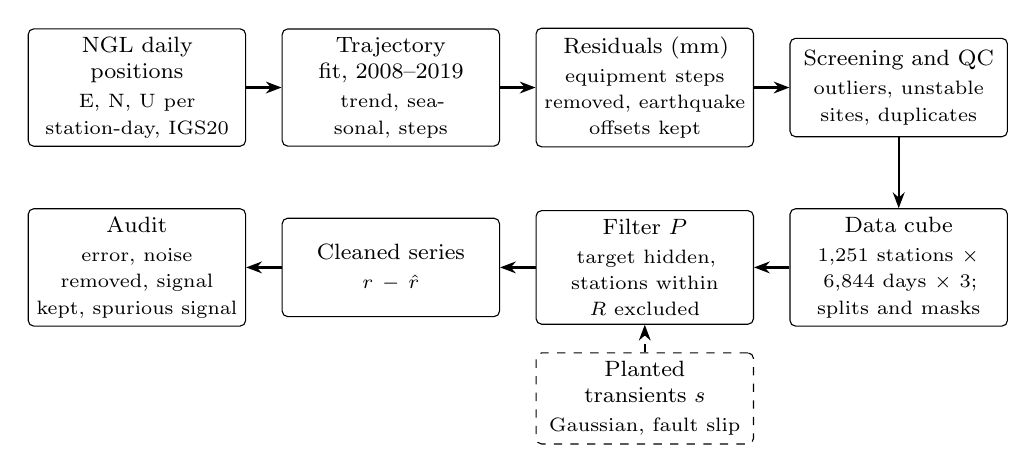
\begin{tikzpicture}[
        box/.style={draw, rounded corners=2pt, align=center, font=\footnotesize, minimum height=1.25cm, text width=2.55cm, inner sep=3pt},
        arr/.style={-{Stealth[length=2mm]}, thick},
      node distance=0.45cm]
      \node[box] (raw) {NGL daily positions\\[1pt]{\scriptsize E, N, U per station-day, IGS20}};
      \node[box, right=of raw] (traj) {Trajectory fit, 2008--2019\\[1pt]{\scriptsize trend, seasonal, steps}};
      \node[box, right=of traj] (res) {Residuals (mm)\\[1pt]{\scriptsize equipment steps removed, earthquake offsets kept}};
      \node[box, right=of res] (qc) {Screening and QC\\[1pt]{\scriptsize outliers, unstable sites, duplicates}};
      \node[box, below=0.9cm of qc] (cube) {Data cube\\[1pt]{\scriptsize 1,251 stations $\times$ 6,844 days $\times$ 3; splits and masks}};
      \node[box, left=of cube] (filt) {Filter $P$\\[1pt]{\scriptsize target hidden, stations within $R$ excluded}};
      \node[box, left=of filt] (clean) {Cleaned series\\[1pt]{\scriptsize $r - \hat r$}};
      \node[box, left=of clean] (audit) {Audit\\[1pt]{\scriptsize error, noise removed, signal kept, spurious signal}};
      \node[box, below=0.35cm of filt, minimum height=0.8cm, dashed] (plant) {Planted transients $s$\\[1pt]{\scriptsize Gaussian, fault slip}};
      \draw[arr] (raw) -- (traj); \draw[arr] (traj) -- (res); \draw[arr] (res) -- (qc); \draw[arr] (qc) -- (cube);
      \draw[arr] (cube) -- (filt); \draw[arr] (filt) -- (clean); \draw[arr] (clean) -- (audit);
      \draw[arr, dashed] (plant) -- (filt);
  \end{tikzpicture}}
  \caption{Processing chain from daily GNSS positions to the signal-loss audit. \towrite{Check caption.}}
  \label{fig:pipeline}
\end{figure}

\subsection{Data}

% P2: What the data are physically: NGL daily IGS20 solutions; per station and
%     day, antenna position (m) E/N/U relative to a reference point, from 24 h
%     of observations; formal 1-sigma ~1 mm horizontal, 3-5 mm vertical. A
%     three-component displacement series sampled daily: periods 2 days to
%     decades, below the seismic band; no instrument response.
%     Noise character in this region: white plus flicker and random-walk
%     (temporally correlated) noise, langbein2008.
%     cite: ngl2026, langbein2008
\towrite{Paragraph 2: what one daily solution is.}

% P3: Selection: box 32.4-42.1 N, 124.6-114.0 W; >=1,095 daily solutions;
%     1,381 stations; from 2008. Removed 130: 30 with <1 year after 2008;
%     22 non-tectonic site motion (robust scale >10 mm horizontal or >30 mm
%     vertical; e.g. Central Valley subsidence); 78 co-located duplicates
%     within 1 km. Left: 1,251 stations, 6.45e6 station-days, 6,844 days
%     (2008-01-01 to 2026-09-26). Median nearest-neighbour distance 9.7 km
%     (2018); a typical station has 23 neighbours within 50 km, 75 within 100.
%     Figure 2a.
\towrite{Paragraph 3: station selection and the network (Fig.~\ref{fig:network}a).}

\begin{figure}[t]
  \centering
  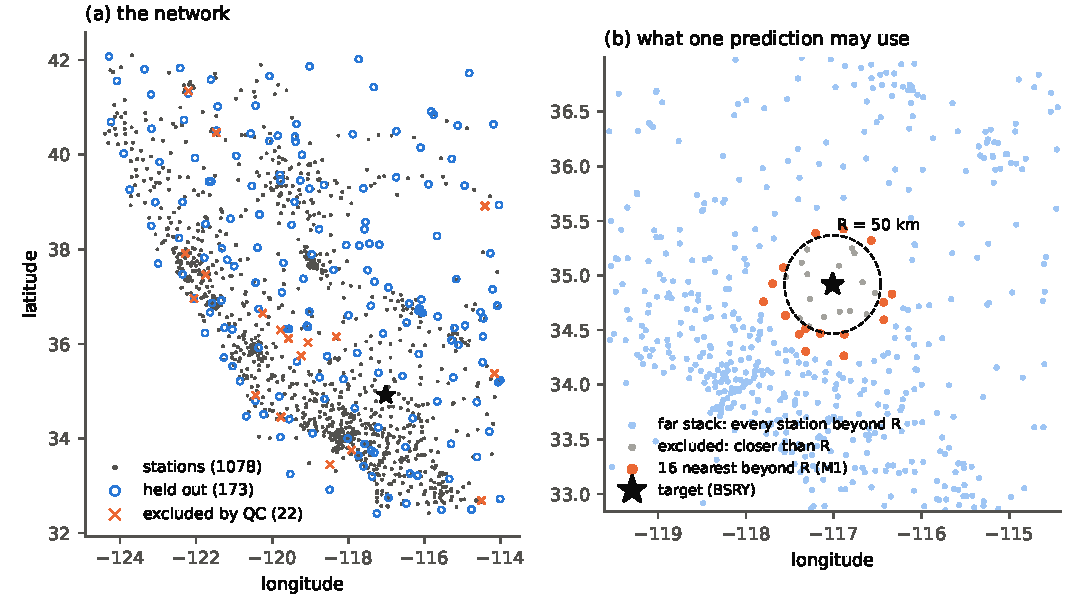
\includegraphics[width=\textwidth]{figures/network.pdf}
  \caption{(a) Stations used, held out and excluded. (b) What a prediction for one target may use at $R = 50$~km. \towrite{Expand caption.}}
  \label{fig:network}
\end{figure}

\subsection{From positions to residuals}

% P4: Why residuals: plate motion is tens of mm/yr (~370 mm east over 18 years
%     at BSRY, Fig. 3a) and seasonal cycles several mm; transients are mm-cm.
%     A dominant trend also defeats source-separation methods unless it is
%     removed first (gualandi2016, pp. 335, 338).
%     Trajectory model, Eq. (1): constant, rate, annual and semi-annual
%     harmonics, Heaviside steps at catalogued epochs; fitted on 2008-2019 only
%     and extrapolated, so no evaluation day influences it.
\towrite{Paragraph 4: the trajectory model and why it is fitted on the training years only.}

\begin{equation}
  x_{i,c}(t) = a + v\,(t - t_0) + \sum_{k=1}^{2}\left[s_k \sin(2\pi k t) + c_k \cos(2\pi k t)\right] + \sum_{j} b_j\, H(t - t_j) + r_{i,c}(t)
  \label{eq:trajectory}
\end{equation}

% P5: Steps: equipment changes removed (artefacts; after 2019 with a local
%     +-30-day estimate). Earthquake offsets kept: real, coherent deformation a
%     filter should preserve. Fig. 3b: El Mayor-Cucapah 2010 and Ridgecrest
%     2019 offsets remain, with postseismic drift after Ridgecrest.
\towrite{Paragraph 5: equipment steps removed, earthquake offsets kept (Fig.~\ref{fig:processing}b).}

% P6: Screening and QC: >5 robust sigma from a 61-day running median -> missing;
%     unstable stations removed (above); scoring QC after 2019 (scatter up >3x,
%     or unexplained jump >50 mm horizontal / 100 mm vertical) -> not scored.
\towrite{Paragraph 6: outlier screening and quality control.}

% P7: The data cube and partition: residuals + sigma + availability, 1,251 x
%     6,844 x 3. Train 2008-2019, validation 2020-2021 (all decisions), test
%     2022 onward (reporting). 173 stations held out by farthest-point sampling.
%     Ridgecrest: 150 km, Jul 2019-Jun 2020 excluded from training. Learned
%     models train on "quiet" residuals: training-fit earthquake offsets
%     subtracted, +-30 days of M>=6 skipped, normalised by station noise scale.
\towrite{Paragraph 7: the data cube, splits and held-out stations.}

% P8: Why displacement and not rates: differencing is a high-pass filter; 2 cm
%     of afterslip over a year is ~0.05 mm/day against ~1.5 mm daily scatter.
%     Increments are an extra input to the attention network for onsets.
\towrite{Paragraph 8: why we filter displacement rather than rates.}

\begin{figure}[t]
  \centering
  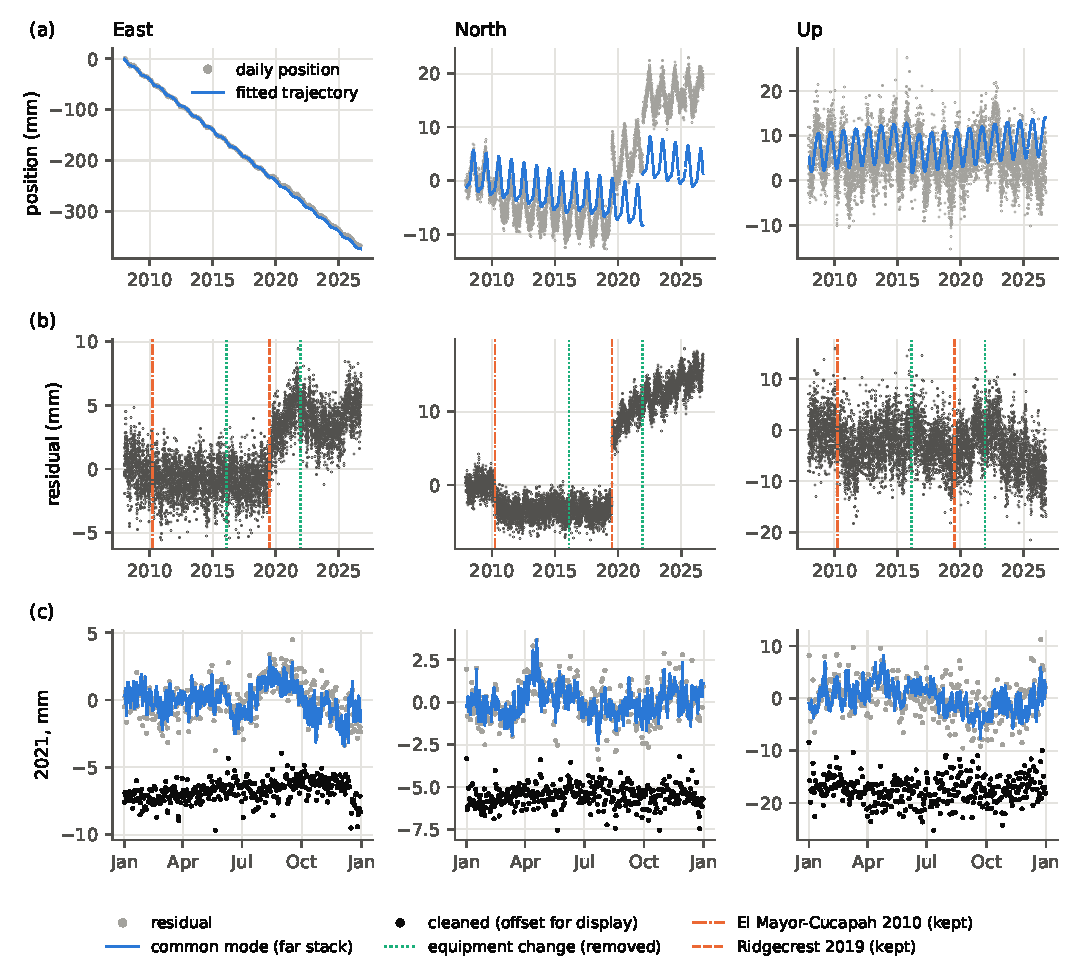
\includegraphics[width=\textwidth]{figures/data_processing.pdf}
  \caption{From positions to residuals at station BSRY. \towrite{Expand caption: (a) positions and trajectory, (b) residual, (c) one validation year with the network common mode and the cleaned series.}}
  \label{fig:processing}
\end{figure}

%% ===========================================================================
\section{The signal-loss audit}
\label{sec:audit}
%% ===========================================================================

\subsection{Leave-one-out filtering and the exclusion radius}

% P1: A filter P estimates the shared part, r_hat = P(r); cleaned = r - r_hat.
%     Leave-one-out filters never read the target; stations within R are
%     excluded (Fig. 2b). One pass cleans every station. Target-inclusive
%     filters audited the same way but not scored on error (reading the target
%     is trivially rewarded). Leak checks: hidden or forbidden values poisoned
%     with 1e6 mm must not change predictions; run for every model.
\towrite{Paragraph 1: leave-one-out, the exclusion radius $R$ and leak checks.}

\subsection{Four measures}

% P2: Reconstruction error: leave-one-out error on validation days, split into
%     fast (error minus its 61-day running median) and slow; normalised by the
%     station's robust training-period scale; median over stations; zero
%     prediction scores 0.723 (val). Fast part is the primary score.
\towrite{Paragraph 2: reconstruction error.}

% P3: Noise removed: per station 1 - rms(fast(r - r_hat)) / rms(fast(r)),
%     averaged over E/N/U, median over stations. Same for every filter,
%     including target-inclusive ones.
\towrite{Paragraph 3: noise removed.}

% P4: Signal kept (retention), Eq. (2): plant s, filter with and without it,
%     Delta = (r + s - P(r + s)) - (r - P(r)), rho = <Delta, s>/<s, s> over
%     horizontal components, the transient's days and nearby stations. Pairing
%     removes the noise term; for linear P, rho = <s - P(s), s>/<s, s>.
%     Fig. 4 illustrates.
\towrite{Paragraph 4: signal kept.}

\begin{equation}
  \rho = \frac{\langle \Delta,\, s \rangle}{\langle s,\, s \rangle},\qquad
  \Delta = \big(r + s - P(r+s)\big) - \big(r - P(r)\big)
  \label{eq:retention}
\end{equation}

% P5: Spurious signal: largest change at stations outside the transient that
%     it can still affect through their neighbours, as a fraction of its
%     amplitude (largest station displacement for events).
\towrite{Paragraph 5: spurious signal.}

\subsection{Planted and real signals}

% P6: Gaussian transients: s = A exp(-d^2/2L^2) g(t) u; A 2-10 mm, L 10-100 km,
%     duration 10-90 days, raised-cosine rise, 60-day hold, fall; centres at
%     random scored stations; packed into runs so that no station is affected
%     by two transients. 720 per filter in validation (20 per grid cell).
\towrite{Paragraph 6: Gaussian transients.}

% P7: Fault-slip events: SCEC CFM 7.0 surfaces (UTM 11, NAD27); triangular
%     dislocations in an elastic half-space, Poisson 0.25; random suitable
%     fault and along-strike position. Templates with ranges from full texts:
%     - shallow slow slip: 8-25 km, surface to 2-4 km, 8-45 mm, front
%       0.4-9 km/day, local rise 1-8 days (materna2024, vavra2024);
%     - afterslip: 15-50 km, top 0-2 km, bottom 5-12 km, 10-40 cm, log decay
%       tau 17-34 days, 365 days (gonzalezortega2014).
%     Kept only if >=3 scored stations move >1 mm (visible: 15% of slow-slip
%     placements, 93% of afterslip). 20 of each; identical across filters.
%     Triggered creep (ramos2020, xu2020) dropped: 1 of 300 placements visible.
%     Limitations: elastic half-space; uniform tapered slip; afterslip without
%     its earthquake; placed on any steep fault of the right style.
%     cite: plesch2007, plesch2024cfm, nikkhoo2015
\towrite{Paragraph 7: fault-slip events from the event library.}

% P8: Real earthquake offsets: every catalogued earthquake step in the scoring
%     years at scored stations; offset = mean of 10 days after minus 10 days
%     before, horizontal; kept = <kept, observed>/<observed, observed>; only
%     offsets >=3 mm with no other step within 15 days. 703 catalogued steps
%     in the validation years (mainly 2020 Monte Cristo Range M6.5, 2021
%     Antelope Valley M6.0, 2021 Petrolia M6.2), 37 scored. No ground truth:
%     the observed offset includes noise. Ridgecrest postseismic retention.
\towrite{Paragraph 8: real earthquake offsets and Ridgecrest.}

\begin{figure}[t]
  \centering
  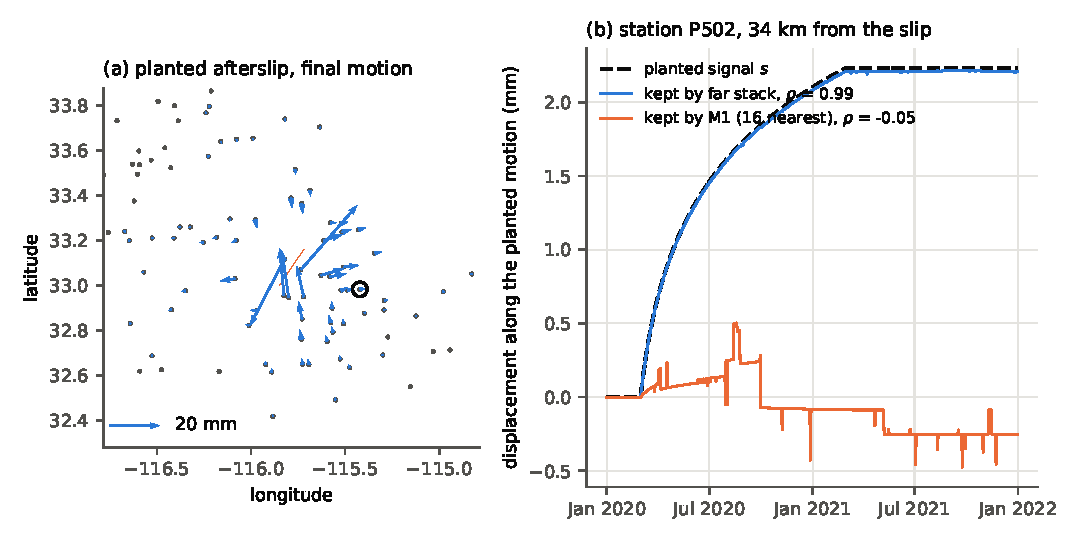
\includegraphics[width=\textwidth]{figures/audit.pdf}
  \caption{Measuring signal kept. \towrite{Expand caption; note that P502 is the median station among 17 at 15--40~km.}}
  \label{fig:audit}
\end{figure}

\subsection{Protocol}

% P9: All decisions on validation years; results reported on test years after
%     freezing the method [date]; paired block bootstrap (30-day blocks and
%     stations) for error, bootstrap over planted transients for signal kept;
%     learned models with five seeds.
\towrite{Paragraph 9: decisions, freeze date, bootstrap, seeds.}

%% ===========================================================================
\section{Filters}
\label{sec:filters}
%% ===========================================================================

% P1: Three families (Table 1): target-inclusive (C1, C3, M2-self) = common
%     practice; distance-excluded (far stack, D1 = the 400 km design of
%     bachelot2025, as described in their paper); leave-one-out models over
%     nearest neighbours (M1-M4) and learned models (M3k, M5, M5-aug).
\towrite{Paragraph 1: the three families.}

% P2: Classical and regression filters, one or two sentences each:
%     C1 network mean (wdowinski1997); C3 sub-regional probabilistic PCA,
%     swept 1/4/8 regions x 1-3 components (tipping1999, gruszczynski2018,
%     liu2026); M2 robust weighted median after kreemer2021, M2-self including
%     the target; M1 distance-weighted mean, 16/64/256 neighbours; M3 ridge
%     regression (per station and pooled), inputs rescaled by available
%     neighbours; M4 band-split ridge (7/60/400-day bands), gaps filled from
%     each station's own series.
\towrite{Paragraph 2: classical and regression filters.}

% P3: Learned models: M3k learned kernel (MLP of distance, azimuth, noise level
%     -> weight; 1,411 parameters; 16 or 256 neighbours). M5: divided
%     space-time attention over 64 days, conv patch stem, 32 nearest neighbours
%     plus the far stack as a summary node, output a correction to the far
%     stack; 212k parameters. M5-aug: Gaussian and dipole fields added to
%     inputs (not targets) in half the training samples.
\towrite{Paragraph 3: learned models.}

\begin{table}[t]
  \centering
  \small
  \caption{Filters audited. \towrite{Check descriptions.}}
  \label{tab:filters}
  \begin{tabular}{p{2.1cm}p{8.6cm}r}
    \toprule
    Name & Description & Parameters \\
    \midrule
    \multicolumn{3}{l}{\textit{Target-inclusive}} \\
    C1 & Mean of the whole network, target included & 0 \\
    C3 & Sub-regional probabilistic PCA; 1, 4 or 8 regions $\times$ 1--3 components & $\sim$3.7k/comp. \\
    M2-self & Robust weighted median of the 16 nearest and the target & 2 \\
    \multicolumn{3}{l}{\textit{Distance-excluded}} \\
    Far stack & Mean of every station beyond $R$; D1 at $R = 400$~km & 0 \\
    \multicolumn{3}{l}{\textit{Leave-one-out over nearest neighbours}} \\
    M1 & Distance-weighted mean of the 16 (64, 256) nearest beyond $R$ & 1 \\
    M2 & Robust weighted median of the 16 nearest beyond $R$ & 2 \\
    M3a / M3b & Ridge regression on 16 neighbours, per station / pooled & 65/station; 257 \\
    M4a / M4b & M3 per time band (under 7, 7--60, 60--400, over 400 days) & 4 $\times$ M3 \\
    \multicolumn{3}{l}{\textit{Learned}} \\
    M3k & Learned kernel: neighbour weight from distance, azimuth and noise level; 16 or 256 neighbours & 1,411 \\
    M5 & Space--time attention: 32 neighbours and the far stack, 64-day window & 212,048 \\
    M5-aug & M5 trained with planted transients in its inputs & 212,048 \\
    \bottomrule
  \end{tabular}
\end{table}

%% ===========================================================================
\section{Results}
\label{sec:results}
%% ===========================================================================

% All numbers below are validation-year values ("val") until the test-year
% runs; Table 2 will be regenerated from the results files.

\subsection{The trade-off between noise removed and signal kept}

% P1: Main figure (Fig. 5). Noise removed (x) vs signal kept for 100 km
%     transients (y), one point per filter at R = 0, lines through the radius
%     sweeps. Numbers (val): far stack 26.6% / 0.83; C1 26.7% / 0.83;
%     M1 22.2% / 0.00; M1-256 26.4% / 0.21; M3k-256 27.1% / 0.22;
%     M5 26.8% / 0.56; M5-aug 26.5% / 0.80; D1 24.9% / 1.00.
%     Message: the far stack and C1 sit at the top right; the nearest-neighbour
%     filters lose signal at similar or lower noise removal.
\towrite{Paragraph 1: the overall trade-off (Fig.~\ref{fig:tradeoff}).}

\begin{figure}[t]
  \centering
  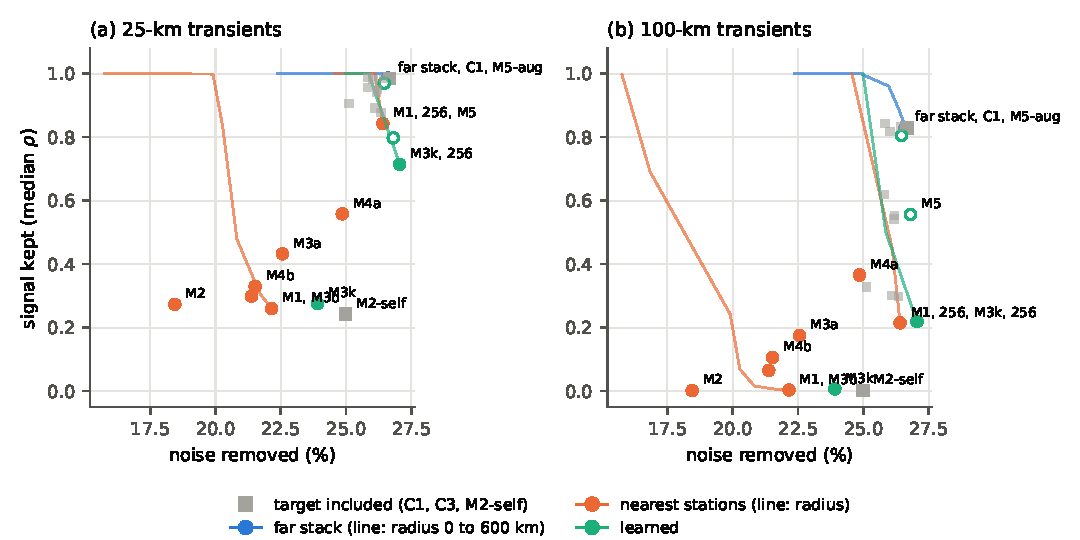
\includegraphics[width=\textwidth]{figures/tradeoff.pdf}
  \caption{\towrite{Caption.}}
  \label{fig:tradeoff}
\end{figure}

% P2: The exclusion radius trades signal kept against spurious signal; no
%     best radius. Far stack R = 0 -> 400 km: 100-km kept 0.83 -> 1.00,
%     spurious 0.11 -> 0.24, noise removed 26.6% -> 24.9% (val).
\towrite{Paragraph 2: what the radius does.}

\subsection{Number of stations versus distance}

% P3: (Fig. 6) Error at R = 0 (val): M1 16 / 64 / 256 neighbours 0.531 /
%     0.511 / 0.507; far stack (all 1,250) 0.509. At R = 100: 0.561 (16),
%     0.515 (256), 0.512 (far stack). 25-km blobs kept by M1: 0.26 (16) ->
%     0.84 (256). Interpretation: shared noise is network-wide, averaging
%     error falls with the number of stations; distance matters modestly once
%     enough stations are averaged. Compare tianshen2016 (correlation vs
%     distance).
\towrite{Paragraph 3: count beats distance (Fig.~\ref{fig:count}).}

% P3b: Regression on the same 16 neighbours (val, R = 0). Error: M3a 0.527,
%     M3b 0.534, M4a 0.517, M4b 0.532 (M1 0.531): per-station weights (a) beat
%     pooled ones (b); band splitting helps M4a. Signal kept, 25 / 100 km:
%     M3a 0.43 / 0.17, M3b 0.30 / 0.07, M4a 0.56 / 0.37, M4b 0.33 / 0.11
%     (M1 0.26 / 0.00): regression keeps more than the weighted mean of the
%     same stations, but far less than the far stack (0.99 / 0.83).
%     Afterslip 15-40 km: M3a 0.22, M3b 0.24, M4a 0.53, M4b 0.31.
%     Possible reason for M4a (to check before claiming): its long-period
%     bands are weighted separately and can down-weight shared slow signal.
\towrite{Paragraph 3b: regression on the nearest stations (M3, M4).}

\begin{figure}[t]
  \centering
  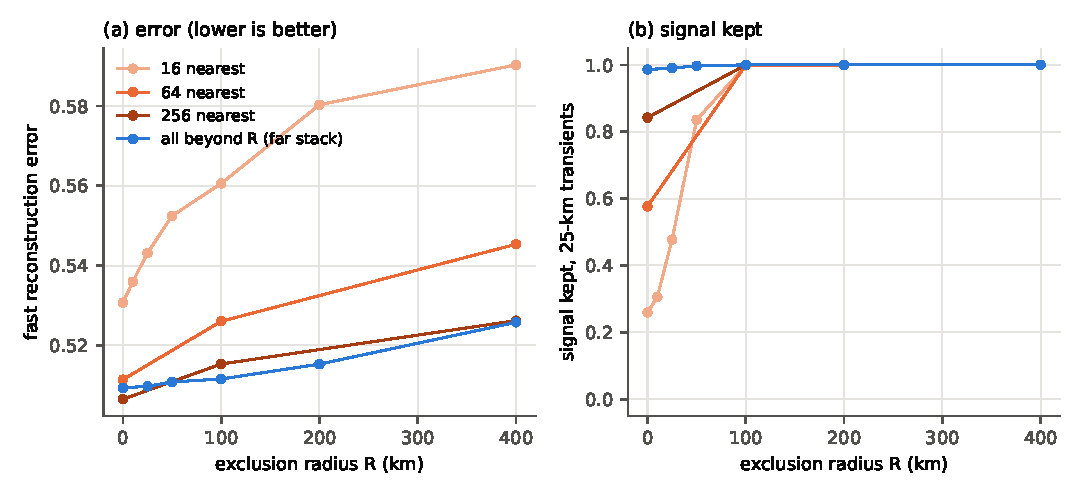
\includegraphics[width=\textwidth]{figures/count_vs_distance.pdf}
  \caption{\towrite{Caption.}}
  \label{fig:count}
\end{figure}

\subsection{Realistic transients}

% P4: (Fig. 7) Afterslip kept by distance from the slipping patch (val):
%     within 5 km M1 0.96; 15-40 km M1 0.09, M3k 0.11, M2 0.23, M3a 0.22,
%     M3b 0.24, M4a 0.53, M4b 0.31, M3k-256 0.73, M1-256 0.96, M5 0.87,
%     M5-aug 0.99, far stack 1.00; >40 km M1 -0.05, M4a 0.42, M3k-256 0.46,
%     far stack 0.99.
%     Mechanism: opposite motion across the fault cancels in a near-fault
%     neighbour average; farther away all neighbours move together.
%     Gaussian transients are pessimistic near faults, optimistic in the far
%     field.
\towrite{Paragraph 4: near field kept, far field removed (Fig.~\ref{fig:distance}).}

% P5: Shallow slow slip (val): seen by a median of 4 stations within ~5 km,
%     largest motion ~4.7 mm; kept by nearly all filters (0.97-1.00), but
%     spread into neighbours: spurious 0.10 (M1), 0.21 (M2), 0.29 (M2-self),
%     0.08 (M3k), 0.08-0.09 (M3, M4), 0.00 (far stack).
\towrite{Paragraph 5: shallow slow slip and the spurious signal it causes.}

\begin{figure}[t]
  \centering
  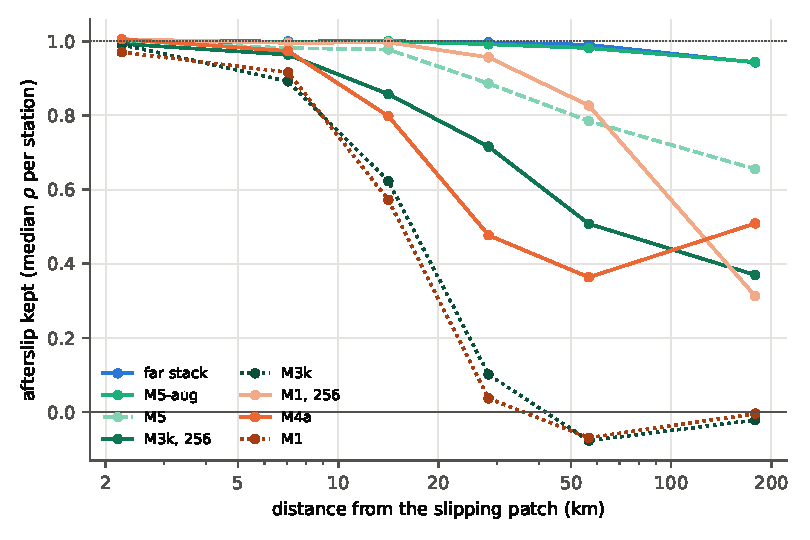
\includegraphics[width=0.8\textwidth]{figures/distance_from_fault.pdf}
  \caption{\towrite{Caption.}}
  \label{fig:distance}
\end{figure}

\subsection{Real earthquake offsets}

% P6: (Fig. 8) 37 real offsets (val), median kept: far stack 0.98, C1 0.98,
%     D1 0.99, M5-aug 0.98, M3k-256 0.88, M5 0.88, M1-256 0.83, M3k 0.81,
%     M3a 0.77, M4a 0.75, M3b 0.74, M1 0.72, M4b 0.72, M2 0.69, M2-self 0.60;
%     C3 0.90-0.95. Same ranking as the planted signals: the planted tests are
%     not misleading. Caveat: no ground truth. Ridgecrest numbers: to collect.
\towrite{Paragraph 6: real offsets confirm the planted results (Fig.~\ref{fig:real}).}

\begin{figure}[t]
  \centering
  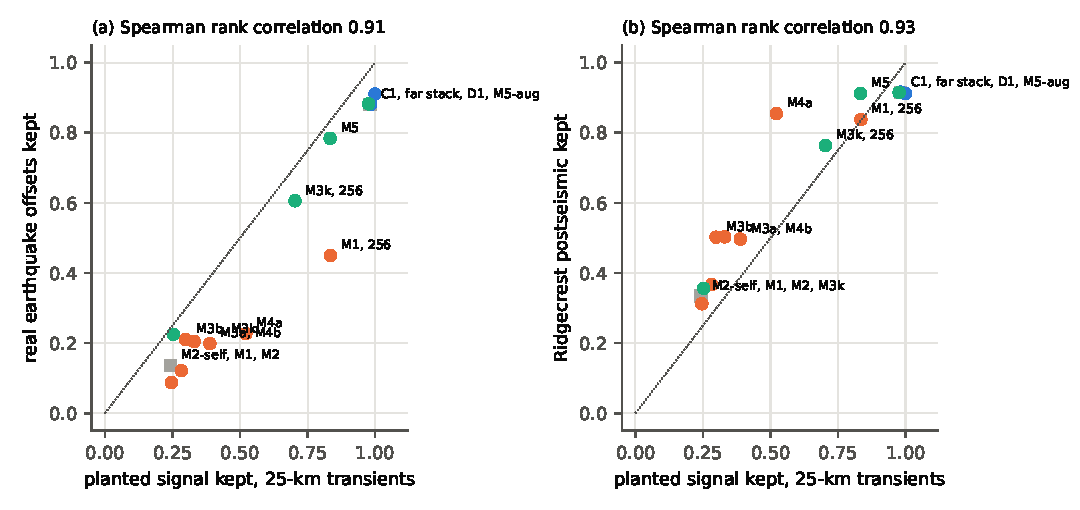
\includegraphics[width=\textwidth]{figures/planted_vs_real.pdf}
  \caption{\towrite{Caption.}}
  \label{fig:real}
\end{figure}

\subsection{Learned models}

% P7: Learned kernel vs fixed weights (16 neighbours, R = 0, val): error
%     0.522 vs 0.536 on the bootstrap blocks, 95% interval of the difference
%     0.008-0.021; signal kept indistinguishable at every width. Learning the
%     weights helps at no cost. The kernel: peaked within ~10 km, flat beyond;
%     noisy neighbours down-weighted ~1/scale^2 (figure in supplement?).
\towrite{Paragraph 7: the learned kernel.}

% P8: Over 256 neighbours M3k has the lowest error (0.4985, 5 seeds, spread
%     0.001) and most noise removed (27.1%), but keeps 0.44 of 50-km and 0.22
%     of 100-km transients against 0.94 / 0.83 for the far stack (bootstrap:
%     error difference vs far stack 0.001-0.015; at R = 100 not
%     distinguishable). Gains over the network mean come from nearby stations.
\towrite{Paragraph 8: more neighbours, more noise removed, less signal kept.}

% P9: M5 (val): error 0.504, noise removed 26.8%, 100-km kept 0.56, afterslip
%     15-40 km 0.87, real offsets 0.88. M5-aug: 0.508, 26.5%, 0.80, 0.99, 0.98.
%     Augmentation restores signal kept for 0.3 points of noise removal;
%     matches the far stack, does not exceed it. [seeds and bootstrap to add]
\towrite{Paragraph 9: the attention network with and without planted-transient training.}

\begin{table}[t]
  \centering
  \small
  \caption{Main results at $R = 0$ unless stated. \textit{Validation years; to be replaced by test-year results after the method freeze.} Error: fast leave-one-out error (lower is better; zero prediction 0.723). Kept: median retention of 25- and 100-km Gaussian transients; afterslip at 15--40~km from the patch; real earthquake offsets.}
  \label{tab:results}
  \resizebox{\textwidth}{!}{%
    \begin{tabular}{lcccccc}
      \toprule
      Filter & Error & Noise removed & Kept 25 / 100 km & Spurious & Afterslip & Real offsets \\
      \midrule
      C1 & -- & 26.7\% & 0.99 / 0.83 & 0.11 & 1.00 & 0.98 \\
      C3 (9 settings) & -- & 25.1--26.4\% & 0.88--0.99 / 0.30--0.84 & 0.27--1.52 & 0.97--1.00 & 0.90--0.95 \\
      M2-self & -- & 25.0\% & 0.24 / 0.00 & 0.10 & 0.19 & 0.60 \\
      Far stack & 0.509 & 26.6\% & 0.99 / 0.83 & 0.11 & 1.00 & 0.98 \\
      D1 ($R = 400$~km) & 0.526 & 24.9\% & 1.00 / 1.00 & 0.24 & 1.00 & 0.99 \\
      M1 & 0.531 & 22.2\% & 0.26 / 0.00 & 0.02 & 0.09 & 0.72 \\
      M1, 256 & 0.507 & 26.4\% & 0.84 / 0.21 & 0.10 & 0.96 & 0.83 \\
      M2 & 0.558 & 18.4\% & 0.27 / 0.00 & 0.11 & 0.23 & 0.69 \\
      M3a & 0.527 & 22.6\% & 0.43 / 0.17 & 0.04 & 0.22 & 0.77 \\
      M3b & 0.534 & 21.4\% & 0.30 / 0.07 & 0.04 & 0.24 & 0.74 \\
      M4a & 0.517 & 24.9\% & 0.56 / 0.37 & 0.03 & 0.53 & 0.75 \\
      M4b & 0.532 & 21.5\% & 0.33 / 0.11 & 0.04 & 0.31 & 0.72 \\
      M3k & 0.517 & 23.9\% & 0.28 / 0.01 & 0.03 & 0.11 & 0.81 \\
      M3k, 256 & 0.499 & 27.1\% & 0.71 / 0.22 & 0.18 & 0.73 & 0.88 \\
      M5 & 0.504 & 26.8\% & 0.80 / 0.56 & 0.15 & 0.87 & 0.88 \\
      M5-aug & 0.508 & 26.5\% & 0.97 / 0.80 & 0.17 & 0.99 & 0.98 \\
      \bottomrule
  \end{tabular}}
\end{table}

%% ===========================================================================
\section{Discussion}
\label{sec:discussion}
%% ===========================================================================

% P1: Practical recommendation: the mean of all stations beyond a modest
%     radius removes about as much noise as any filter tested and keeps
%     transients of all sizes and shapes tested. Report signal kept and
%     spurious signal alongside scatter reduction.
\towrite{Paragraph 1: what practitioners should do.}

% P2: Why local filters remove the far field, and why that matters: the far
%     field constrains depth and moment of slow slip; robust median filters
%     (kreemer2021) and PCA (dong2006; gualandi2016 on PCA mixing sources)
%     behave like local filters in this respect. C3 one-region spurious 1.52.
\towrite{Paragraph 2: why local filters remove the far field and why it matters.}

% P3: Relation to Bachelot et al. (2025): consistent with their finding that
%     excluding nearby stations protects slow slip and that a stack matches the
%     network; adds that the number of stations, not the 400 km distance, is
%     what keeps noise removal high, and that the radius trades signal kept
%     against spurious signal. Neutral wording; their results as reported.
\towrite{Paragraph 3: relation to Bachelot et al.}

% P4: Deep learning: gains in noise removal came from nearby stations;
%     transient-augmented training can teach a network to keep signal without
%     a hand-chosen radius. The bar for future models: more noise removed than
%     the network mean at equal signal kept.
\towrite{Paragraph 4: what this means for deep learning.}

% P5: Limitations: one network (dense, strike-slip, California); elastic
%     half-space and two templates; real offsets without ground truth; daily
%     data only; [validation vs test]. Transfer to sparser networks
%     (Turkiye, median nearest neighbour ~60 km) as future work, with
%     TUSAGA-Aktif data.
\towrite{Paragraph 5: limitations and future work.}

%% ===========================================================================
\section{Conclusions}
\label{sec:conclusions}
%% ===========================================================================

% Four or five sentences mirroring the abstract's findings; no new material.
\towrite{Conclusions: write after the discussion.}

%% ===========================================================================
\section*{Data and code availability}
% NGL data (ngl2026, blewitt2018); SCEC CFM 7.0 (plesch2024cfm); code at the
% GitHub repository (URL, release tag at submission); results files.
\towrite{Data and code availability.}

\section*{Declaration of generative AI in the writing process}
% Elsevier asks for this section. Describe the actual division of work at
% submission (software, analyses, figures, fact-checking vs the writing).
\towrite{AI declaration: write at the end, describing what was actually done.}

\bibliographystyle{elsarticle-harv}
\bibliography{references}

\end{document}
